\documentclass[10pt, handout]{beamer}
\usepackage{xmpincl}
\includexmp{license}
\usepackage[T1]{fontenc}
\usepackage[latin1]{inputenc}
\usepackage{ae}
\usepackage[french]{babel}
\usepackage{array, longtable}
\usetheme{Antibes}
\setbeamertemplate{navigation symbols}{}

% for printing
\usepackage{pgfpages}
\pgfpagesuselayout{2 on 1}[a4paper,border shrink=5mm]
% \pgfpagesuselayout{resize to}[a4paper,border shrink=5mm,landscape]

\title{Computer Science Introductory Course MSC - Software engineering}

\subtitle{Lecture 1: Software Management}
\usepackage{verbatim}

\author[Pablo Oliveira]{Pablo Oliveira \texttt{<pablo@sifflez.org>}}
\institute{ENST}

\date{}

\begin{document}
\begin{frame}
  \titlepage
\end{frame}

\begin{frame}
  \frametitle{Outline}
  \tableofcontents
\end{frame}

\section{Introduction}
\begin{frame}[fragile]
  \frametitle{Lessons from the past}
  \begin{itemize}
  \item 1996 Ariane-5 self-destructs, unhandled floating point exception,
    \$500M lost.
  \item 1998 Mars Climate Orbiter is lost, navigation data expressed in imperial
    units, \$327.6M lost.
  \item 1988-1994 FAA Advanced Automation System, project is abandoned, blame
    on management and over-ambitious specifications, \$2.6B lost.
  \item 1985-1987 Therac-25 medical accelerator, a radiation therapy device
    malfunctions because of a race condition, 5 patients die, others are injured.
  \end{itemize}
\end{frame}

\begin{frame}[fragile]
  \frametitle{Common problems}
  \begin{itemize}
  \item Amount of work is underestimated.
  \item Project specifications are vague.
  \item Lack of communication :
    \begin{itemize}
    \item Communication overheads increase as the number of people increase
      (Brooks)
    \end{itemize}
  \item Issues are not properly tracked.
  \item Teams botch the testing phase because of pressure from management.
  \end{itemize}
\end{frame}

\section{Software life-cycle}

\begin{frame}
  \frametitle{Outline}
  \tableofcontents[currentsection]
\end{frame}

\begin{frame}[fragile]
  \frametitle{Time distribution in a software project ?}
  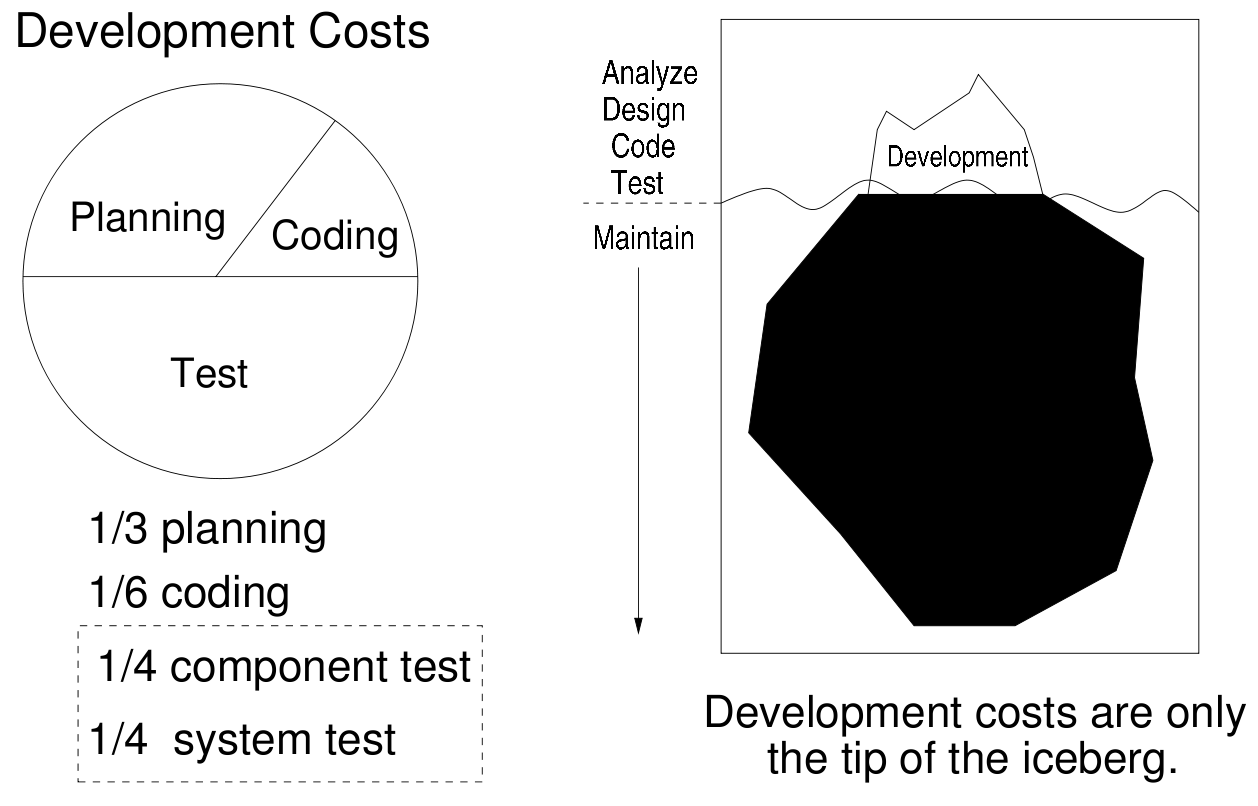
\includegraphics[width=\textwidth]{soft_cost}
  \tiny(source: Nancy Leveson)
\end{frame}

\begin{frame}[fragile]
  \frametitle{Planning}
  \begin{itemize}
  \item Plan time carefully: ``adding manpower to a late software project
    makes it later'' (Brooks).
  \item You only control what you can measure: use metrics.
  \item Model dependencies and deadline, analyse risk.
  \item Keep track of deadlines and critical tasks, Gantt chart.
  \end{itemize}
  \begin{center}
    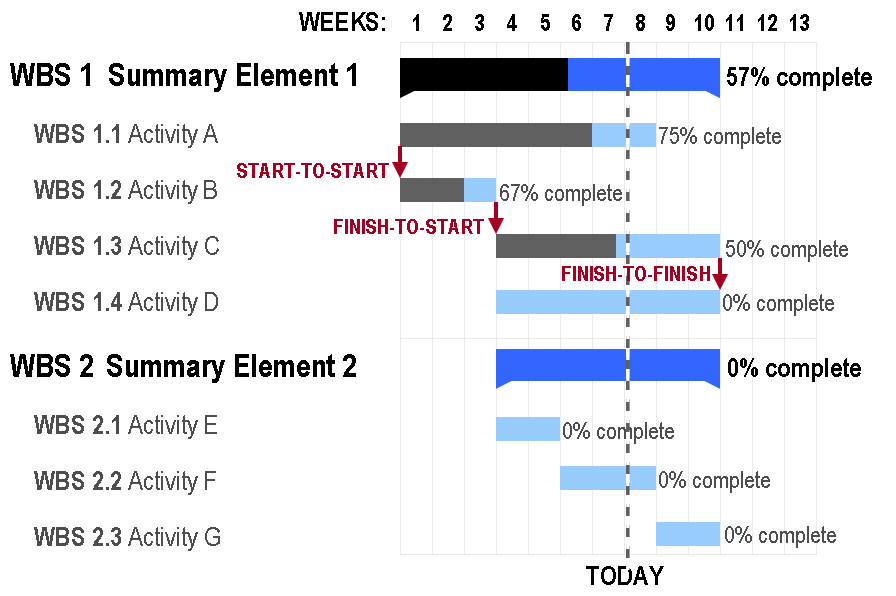
\includegraphics[width=0.4\textwidth]{gantt_chart}
  \end{center}
\end{frame}

\begin{frame}[fragile]
  \frametitle{The phases of software development}
  \begin{itemize}
  \item Analysis (Requirements capture and specification)
  \item Design
  \item Implementation
  \item Integration
  \item Testing
  \item Deployment
  \item Maintenance
  \end{itemize}
\end{frame}

\begin{frame}[fragile]
  \frametitle{Keeping track: Document!}
  \structure{Each software phase should be documented: each component life
    should be traceable}
  \begin{itemize}
  \item Requirements $\longrightarrow$ use-cases, requirements formal document.
  \item Specifications $\longrightarrow$ specifications formal document.
  \item Code $\longrightarrow$ Comments / Revision Control System.
  \item Bugs $\longrightarrow$ Issues tracker / Regressions tests.
  \item User Documentation.
  \end{itemize}
\end{frame}

\section{Requirements capture}

\begin{frame}
  \frametitle{Outline}
  \tableofcontents[currentsection]
\end{frame}

\begin{frame}[fragile]
  \frametitle{Requirements capture}
  \begin{itemize}
  \item Objective: Understand the problem,
    so you can build the system the client needs instead of the system he
    thinks he needs.
  \item Hard because:
    \begin{itemize}
    \item the client may have strong preconceptions about the system.
    \item the client may be vague abouts its needs.
    \end{itemize}
  \item Requirements specify: 'What' a system does and not 'How' it should be
      done.
  \item Requirements should be expressed in a language understandable by the
    client.
  \item Requirements should be traceable.
  \end{itemize}
\end{frame}

\begin{frame}[fragile]
  \frametitle{Requirements analysis}
  \begin{itemize}
  \item Interviewing
    \begin{itemize}
    \item Lots of work
    \item Not necessarily precise
    \end{itemize}
  \item User stories
    \begin{itemize}
    \item Clients write down user stories
    \item Use cases
    \item Each user story has acceptance tests
    \end{itemize}
  \item Straw-men
    \begin{itemize}
    \item Sketch the product
    \item Use anything; napkins, storyboards, HTML, flowcharts
    \item Anything to convey ideas without writing code!
    \end{itemize}
  \item Rapid prototyping
    \begin{itemize}
    \item Create one for client to validate
    \item Major functionality, superficially implemented
    \end{itemize}
  \end{itemize}
\tiny (Source: Irfan Hamid)
\end{frame}

\begin{frame}[fragile]
  \frametitle{Functional Requirements}
  \structure{The functions of a system: what should a system do ?}
  \begin{itemize}
  \item mapping from input to output
  \item control sequencing
  \item timing of functions
  \item handling of exceptional situations
  \item formats of input and output data
  \item real world entities and relationships modeled by the system
  \item ...
  \end{itemize}
\tiny (Source: Steve Easterbrook, University of Toronto)
\end{frame}

\begin{frame}[fragile]
  \frametitle{Non-Functional Requirements}
  \structure{Constraints and quality goals}
  \begin{itemize}
  \item interoperability
  \item portability
  \item availability
  \item safety
  \item ...
  \end{itemize}
\end{frame}

\begin{frame}[fragile]
\frametitle{Requirements specifications}
\begin{itemize}
\item At the end of the requirements gathering phase, the team must produce a
  specification document.
\item The problem must be explained.
\item Functional and Non-Functional requirements must be stated, and numbered.
\item Some exemplary use cases that illustrate the product's functions should be
  given.
\end{itemize}
\end{frame}

\begin{frame}[fragile]
  \frametitle{Requirements must be testable}
  \begin{alertblock}{An untestable requirement}
    The system shall be easy to use by experienced
    controllers and shall be organized in such a way
    that user errors are minimized.
  \end{alertblock}
  \begin{exampleblock}{A testable requirement}
    Experienced controllers shall be able to use all
    the system functions after a total of two hours
    training. After this training, the average number
    of errors made by experienced users shall not
    exceed two per day.
  \end{exampleblock}
  \tiny (Source: Nancy Leveson)
\end{frame}

\begin{frame}[fragile]
  \frametitle{Example of requirements specifications}
  \begin{itemize}
  \item 3.3.4 Intute Repository Search response data
    \begin{itemize}
    \item 3.3.4.1 Description
      The web service must provide responses to name query requests with a list of
      possible matches including the name authority record identifier (URI).
      The service may also need to return all other forms of an entity's name and
      affiliations for further disambiguation.
    \item 3.3.4.2 Related requirements
      3.3.1, 3.2, 3.2.1, 3.2.2.
    \item 3.3.4.3 Source
      Introduced in Stakeholders' Requirements for the Names project prototype
      Intute Repository Search, Page 7.
    \end{itemize}
  \end{itemize}

  \tiny (Source: Software Requirements Specification for the Names project
  prototype \\ by Daniel Needham, Amanda Hill, Alan Danskin \& Stephen Andrews)
\end{frame}

\section{Software Specifications}

\begin{frame}
  \frametitle{Outline}
  \tableofcontents[currentsection]
\end{frame}

\begin{frame}[fragile]
  \frametitle{Specification}
  \begin{itemize}
  \item An abstract description of the software that serves as a
    basis for (or describes) detailed design and implementation
  \item Describes how the requirements will be achieved.
  \item Primary readers will be software designers and
    implementers rather than users or management.
  \item Goals and constraints specified in requirements document
    should be traceable to the design specification (and from
    there to the code.
  \end{itemize}
\tiny (Source: Nancy Leveson)
\end{frame}

\begin{frame}[fragile]
  \frametitle{Views of Specifications}
  \begin{itemize}
  \item Developer
    \begin{itemize}
    \item Must be detailed enough to aid implementation
    \item Must not be ambiguous
    \item Must be traceable
    \end{itemize}
  \item Client
    \begin{itemize}
    \item Must be comprehensible
    \item Must be readable by non-computer specialists
    \end{itemize}
  \item  Legal
    \begin{itemize}
    \item A binding document.
    \item Must contain acceptance (testable) criteria.
    \end{itemize}
  \end{itemize}
  \tiny (Source: Adapted from Irfan Hamid course 2005)
\end{frame}

\begin{frame}[fragile]
  \frametitle{Format of Specifications}
  \begin{itemize}
  \item Natural language (must be as unambiguous as possible)
  \item Semi-formal specifications (UML)
  \item Formal specifications (DFA, Z language, B language, math ...)
  \end{itemize}
\end{frame}

\begin{frame}[fragile]
  \frametitle{Example of specification using: Pre-conditions, Post-conditions, Invariants}
  \begin{verbatim}
   class Dictionnary
       put (x: ELEMENT; key: STRING)
                  require (pre-condition)
                    count <= capacity
                    not key.empty
                  ensure  (post-condition)
                    has (x)
                    item (key) = x
                    count = old count + 1
  invariant
                0 <= count
                count <= capacity
  \end{verbatim}
\end{frame}

\section{Software development models}

\begin{frame}
  \frametitle{Outline}
  \tableofcontents[currentsection]
\end{frame}

\begin{frame}[fragile]
  \frametitle{Waterfall (1/2)}
  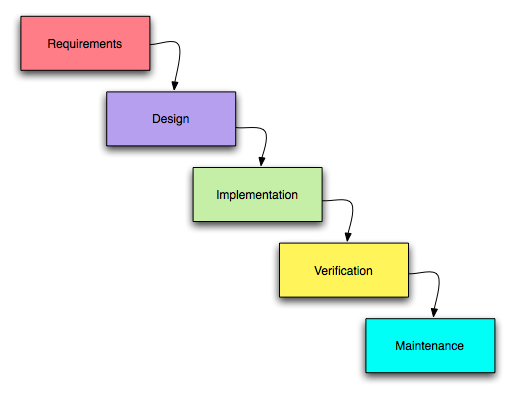
\includegraphics[width=0.8\textwidth]{Waterfall_model}

  \tiny(source: Paul Hoadley)
\end{frame}
\begin{frame}[fragile]
  \frametitle{Waterfall (2/2): pros \& cons}
  \begin{exampleblock}{Pros}
    \begin{itemize}
    \item Disciplined approach.
    \item Big Design Up Front.
    \item Document driven.
    \end{itemize}
  \end{exampleblock}
  \begin{alertblock}{Cons}
    \begin{itemize}
    \item Does not adapt to change:
      \begin{itemize}
      \item Changing requirements.
      \item Problems discovered during the implementation phase.
      \end{itemize}
    \end{itemize}
  \end{alertblock}
\end{frame}


\begin{frame}[fragile]
  \frametitle{V Model (1/2)}
  \begin{center}
    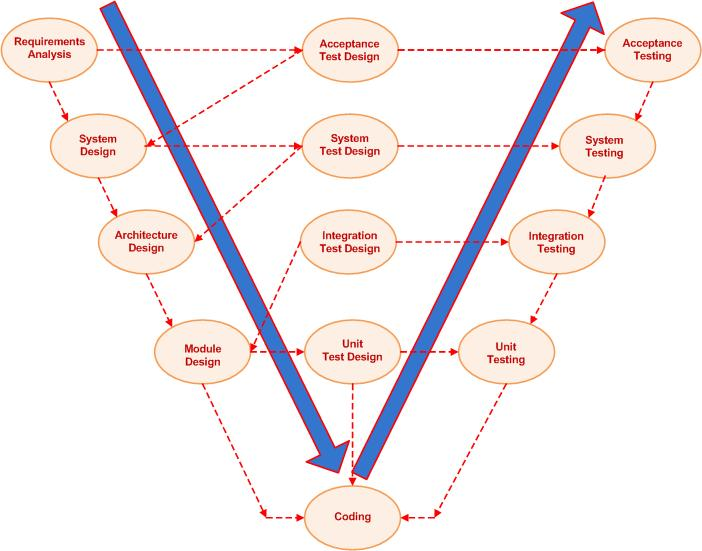
\includegraphics[width=0.8\textwidth]{V-model}
  \end{center}
\end{frame}
\begin{frame}[fragile]
  \frametitle{V Model (2/2)}
  \begin{exampleblock}{}
    \begin{itemize}
    \item Extension of the waterfall model:
      \begin{itemize}
      \item Takes in account the V\&V and defines acceptance tests for each step.
      \end{itemize}
    \item Better correspondence between design \& tests.
    \item Makes V\&V a central part of the process.
    \end{itemize}
  \end{exampleblock}
\end{frame}


\begin{frame}[fragile]
  \frametitle{Evolutionnary}
  \structure {Plan to throw one away}
  \begin{exampleblock}{Pros}
    \begin{itemize}
    \item Test feasibility.
    \item Check requirements.
    \item Discover problems early.
    \item Get user feedback early.
    \end{itemize}
  \end{exampleblock}
  \begin{alertblock}{Cons}
    \begin{itemize}
    \item Prototype gets a life of its own.
    \item Less though out designs.
    \item Less robustness.
    \end{itemize}
  \end{alertblock}
\end{frame}


\begin{frame}[fragile]
  \frametitle{Iterative (1/2)}
  \begin{center}
    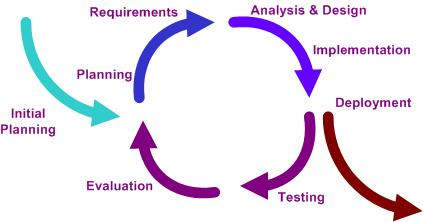
\includegraphics[width=0.7\textwidth]{iterative_model}
  \end{center}
\end{frame}
\begin{frame}[fragile]
  \frametitle{Iterative (2/2): pros \& cons}
  \begin{exampleblock}{Pros}
    \begin{itemize}
    \item Adapts well to change.
    \item Learning from the errors in the previous steps.
    \item Each step produces a finished product.
    \end{itemize}
  \end{exampleblock}
  \begin{alertblock}{Cons}
    \begin{itemize}
    \item Hard to recover from bad design choices in early steps.
    \end{itemize}
  \end{alertblock}
\end{frame}


\begin{frame}[fragile]
  \frametitle{Spiral(1/2)}
  \begin{center}
    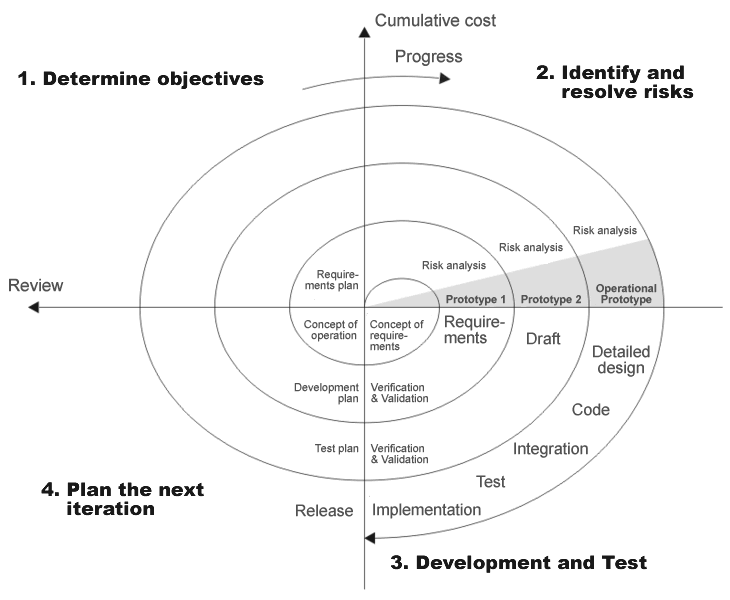
\includegraphics[width=0.7\textwidth]{spiral_model}
  \end{center}

  \tiny (source : Conrad Nutschan)
\end{frame}
\begin{frame}[fragile]
  \frametitle{Spiral(2/2): pros \& cons}
  \begin{exampleblock}{Pros}
    \begin{itemize}
    \item A form of iterative development.
    \item Tries to combines all the previous models.
    \item Risk based.
    \end{itemize}
  \end{exampleblock}
  \begin{alertblock}{Cons}
    \begin{itemize}
    \item Very costly for small projects.
    \end{itemize}
  \end{alertblock}
\end{frame}


\begin{frame}[fragile]
  \frametitle{Agile ?}
  \begin{itemize}
  \item A buzzword that describes an emerging practice of software development.
  \item Encourages adaptation, inspection, communication, customer involvement,
    time-boxed development steps.
  \item Still very new, it is hard to evaluate the benefits from agile methods:
    \begin{itemize}
    \item pair programming.
    \item stand-up meetings.
    \item time-boxed development steps.
    \end{itemize}
  \item Yet it seems mainly effective with small teams of experienced developers.
  \end{itemize}
\end{frame}

\begin{frame}[fragile]
  \frametitle{Which is best ?}
  \begin{itemize}
    \item SE is a young discipline, we lack perspective and objective studies to
      validate its methods.
    \item Depends on the project, the team size and competences, the enterprise
      culture.
    \item Act of faith.
    \item Choose something that works for you, but try to be rigorous and keep
      track of things.
  \end{itemize}
\end{frame}

\section{Software development tools.}

\begin{frame}
  \frametitle{Outline}
  \tableofcontents[currentsection]
\end{frame}

\begin{frame}[fragile]
  \frametitle{Software development tools}
  \begin{itemize}
  \item Tools will never replace team communication.
  \item Tools will never replace well though design.
  \item BUT...
  \item Tools can help in keeping track of code, bugs and issues.
  \item If used wisely, they can ease project documentation,
    management and communication.
  \end{itemize}
\end{frame}
\begin{frame}[fragile]
  \frametitle{Testing frameworks}
  \begin{itemize}
  \item JUnit, ...
  \item Eases writing of unit, functional and regression tests.
  \item Allow automatic execution of the tests.
  \end{itemize}
\end{frame}

\begin{frame}[fragile]
  \frametitle{Version control system}
  \begin{itemize}
  \item SVN(centralized), GIT(distributed), ...
  \item Keep track of changes in code.
  \item Each change is tagged with a commit message that explains which problem
    the code is going to solve.
  \item Developers have the complete history of a line code at their
    fingertips.
  \item When coupled with regression testings, can help finding the exact change
    that introduced a bug.
  \end{itemize}
\end{frame}

\begin{frame}[fragile]
  \frametitle{Issues tracker}
  \begin{itemize}
    \item Roundup, Trac, etc ...
  \item Keep track of issues in a project.
  \item Allow easy bug reporting from users.
  \item Each issue is assigned a ticket which traces:
    \begin{itemize}
    \item the discussion surrounding the issue.
    \item the state of the issue.
    \item the proposed patches to solve the issue.
    \item the code commit that solves the issue.
    \end{itemize}
  \end{itemize}
\end{frame}

\section{References}
\begin{frame}[fragile]
  \frametitle{References}
  \begin{itemize}
    \item Steve Easterbrook, University of Toronto Software Engineering course.
    \item The Mythical Man Month, F. Brooks 1975
    \item The Pragmatic Programmer: From Journeyman to Master, A. Hunt and
      D. Thomas, 1999
    \item Software Engineering: Principles and Practice (2nd edition), H. van Vliet 1999
  \end{itemize}
\end{frame}
\begin{frame}[fragile]
  \begin{center}
    \tiny
    This work is licensed under a Creative Commons Attribution-Noncommercial-Share Alike 3.0 Unported License.
    \vtop{
      \vskip-3ex
      \hbox{
        \includegraphics[height=0.4cm]{cc-logo}
      }
    }
  \end{center}
\end{frame}

\end{document}
